% $Id$

\subsection{Introduction}

GnuPG, also commonly known as GPG, is a free implementation of the
OpenPGP set of cryptography operations from the GNU Project, commonly
available as standard on open source systems such as GNU/Linux and BSD 
distributions.

\subsection{How OpenPGP (and hence GPG) Works}

The OpenPGP set of cryptographic functions include digitally signing and
encrypting a transmission. To perform such tasks, asymmetric key pairs,
commonly referred to as public private keys, are required. These keys
contain user identities (names and email addresses), and are secured 
with a pass-phrase, and are generated by individual users during the 
bootstrapping phase.


Once a user has created a key pair, they must build a Web of Trust 
(WoT), consisting of the public keys of other, trusted users.
Transmissions are encrypted using the public key of the recipient and
the key pair of the sender, ensuring only the sender and recipient are
able to decrypt and/or verify the transmission.


While this system is cryptographically secure, it is only as strong as
the weakest link, which is the human element. Unless 
good password/pass phrase practices\footnote{Eg: periodic changes, use 
of alphanumeric and non alphanumeric characters, not sharing passwords 
or noting passwords down on paper} are employed, a key-pair is only as 
strong as the pass-phrase associated with the keys and how the owner of 
the keys maintains the pass-phrase.


Additionally, a secure method of distributing public keys is required to
ensure a malicious individual does not attempt to alter a public key in
an effort to intercept encrypted communications. To facilitate this, a
network of replicating keyservers is maintained on the Internet, for
simple key management.

\pagebreak 

\subsubsection{The Web Of Trust}

\begin{figure}[ht]

\label{fig:wot}

\begin{center}

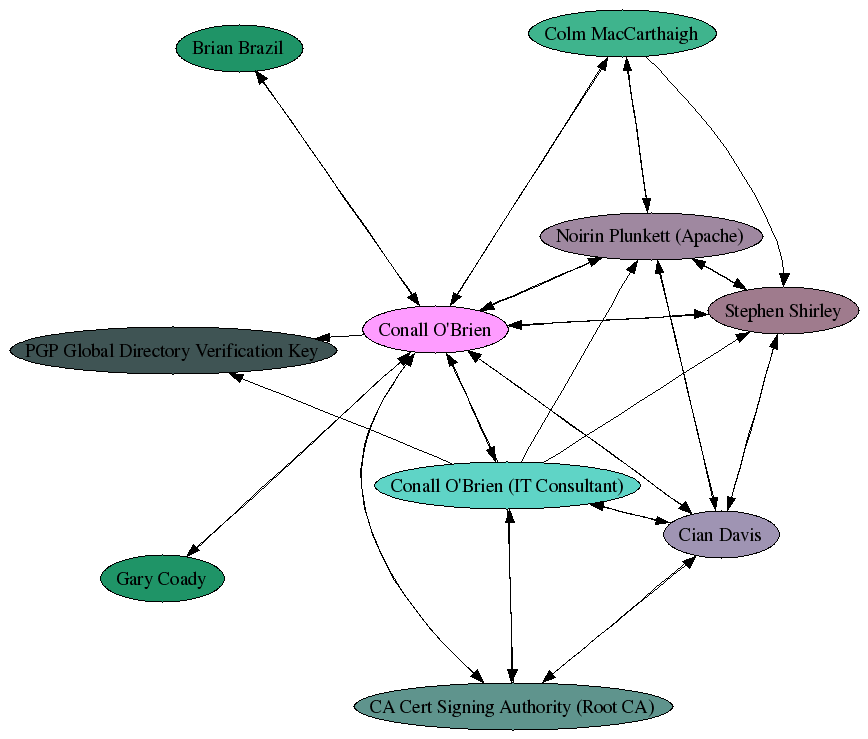
\includegraphics[bb= 0 0 868 739,scale=0.5]{include/EE7DC74E.png}

\end{center}

\caption{Graphical Representation of the WoT for OpenPGP Key 0xEE7DC74E}

\end{figure}

\clearpage

\subsection{Cryptography Algorithms}

The OpenGPG standard encourages the use of the IDEA algorithm, primarily
for backwards compatibility with traditional PGP encryption, before IDEA
was phased out due to patent issues. GnuPG has opted not to use the IDEA
algorithm by default\footnote{Although it can be enabled manually, once an IDEA usage license is purchased},
instead using patent free algorithms such as CAST5, 3DES, AES, Blowfish
and Twofish.

\subsection{Further Information}

Further information about public private key cryptography, including key
management is available in Applied Cryptography by Bruce Sneider.
